\chapter{Integrales de trayectoria	 en espacio plano.}
El formalismo mas común de la mecánica cuantica se deriva de cambiar las variables clasicas de posición y momentum ($p$ y $q$) por operadores que obedecen el álgebra:
\begin{equation}
[\hat{q},\hat{p}]=i\hbar
\end{equation}
Esta relación se conoce como la condción de cuantización de Heisenberg, en general en la mecánica cuantica de operadores estos últimos viven en un espacio de Hilbert.
\\
\\
La formulación de integrales de camino se basa en la noción de \textbf{propagador}, esta función es tal que dada una funcion de onda en un instante de tiempo $t_1$, $\psi(x_1,t_1)$ da la evolucion hasta un instante de tiempo $t_2$, entregando $\psi(x_2,t_2)$. En cierta manera es parecido al principio de Huygens:
\begin{equation}
\psi(x_f,t_f)=\int K(q_f,t_f;q_i,t_i)\psi(q_i,t_i)dq_i
\end{equation}
De acuerdo con la mecánica cuántica $\psi(q_f,t_f)$ representa la probabilidad de que una partícula se encuentre en un punto $q_f$ en el instante de tiempo $t_f$, por tanto $K(q_f,t_f;q_i,t_i)$ representa la amplitud de probabilidad de transición entre un estado ($q_i,t_i$) y ($q_f,t_f$).
\begin{equation}
P(q_f,t_f;q_i,t_i)=\Vert K(q_f,t_f;q_i,t_i) \Vert^2
\end{equation}
Si dividimos el intervalo de tiempo en $t_i\rightarrow t \rightarrow t_f$, tenemos de la definición de $K$:
\begin{eqnarray}
\nonumber \psi(q_f,t_f)&=&\int\int K(q_f,t_f;q,t)K(q,t;q_i,t_i)dqdq_i\\
\Rightarrow K(q_f,t_f;q_i,t_i)&=&\int dq K(q_f,t_f;q,t)K(q,t;q_i,t_i)
\end{eqnarray}
Como ejemplo de lo anterior podemos analizar el experimento de la doble rendija. En la Figura 1 encontramos un esquema de este:
\begin{figure}[h]
\centering
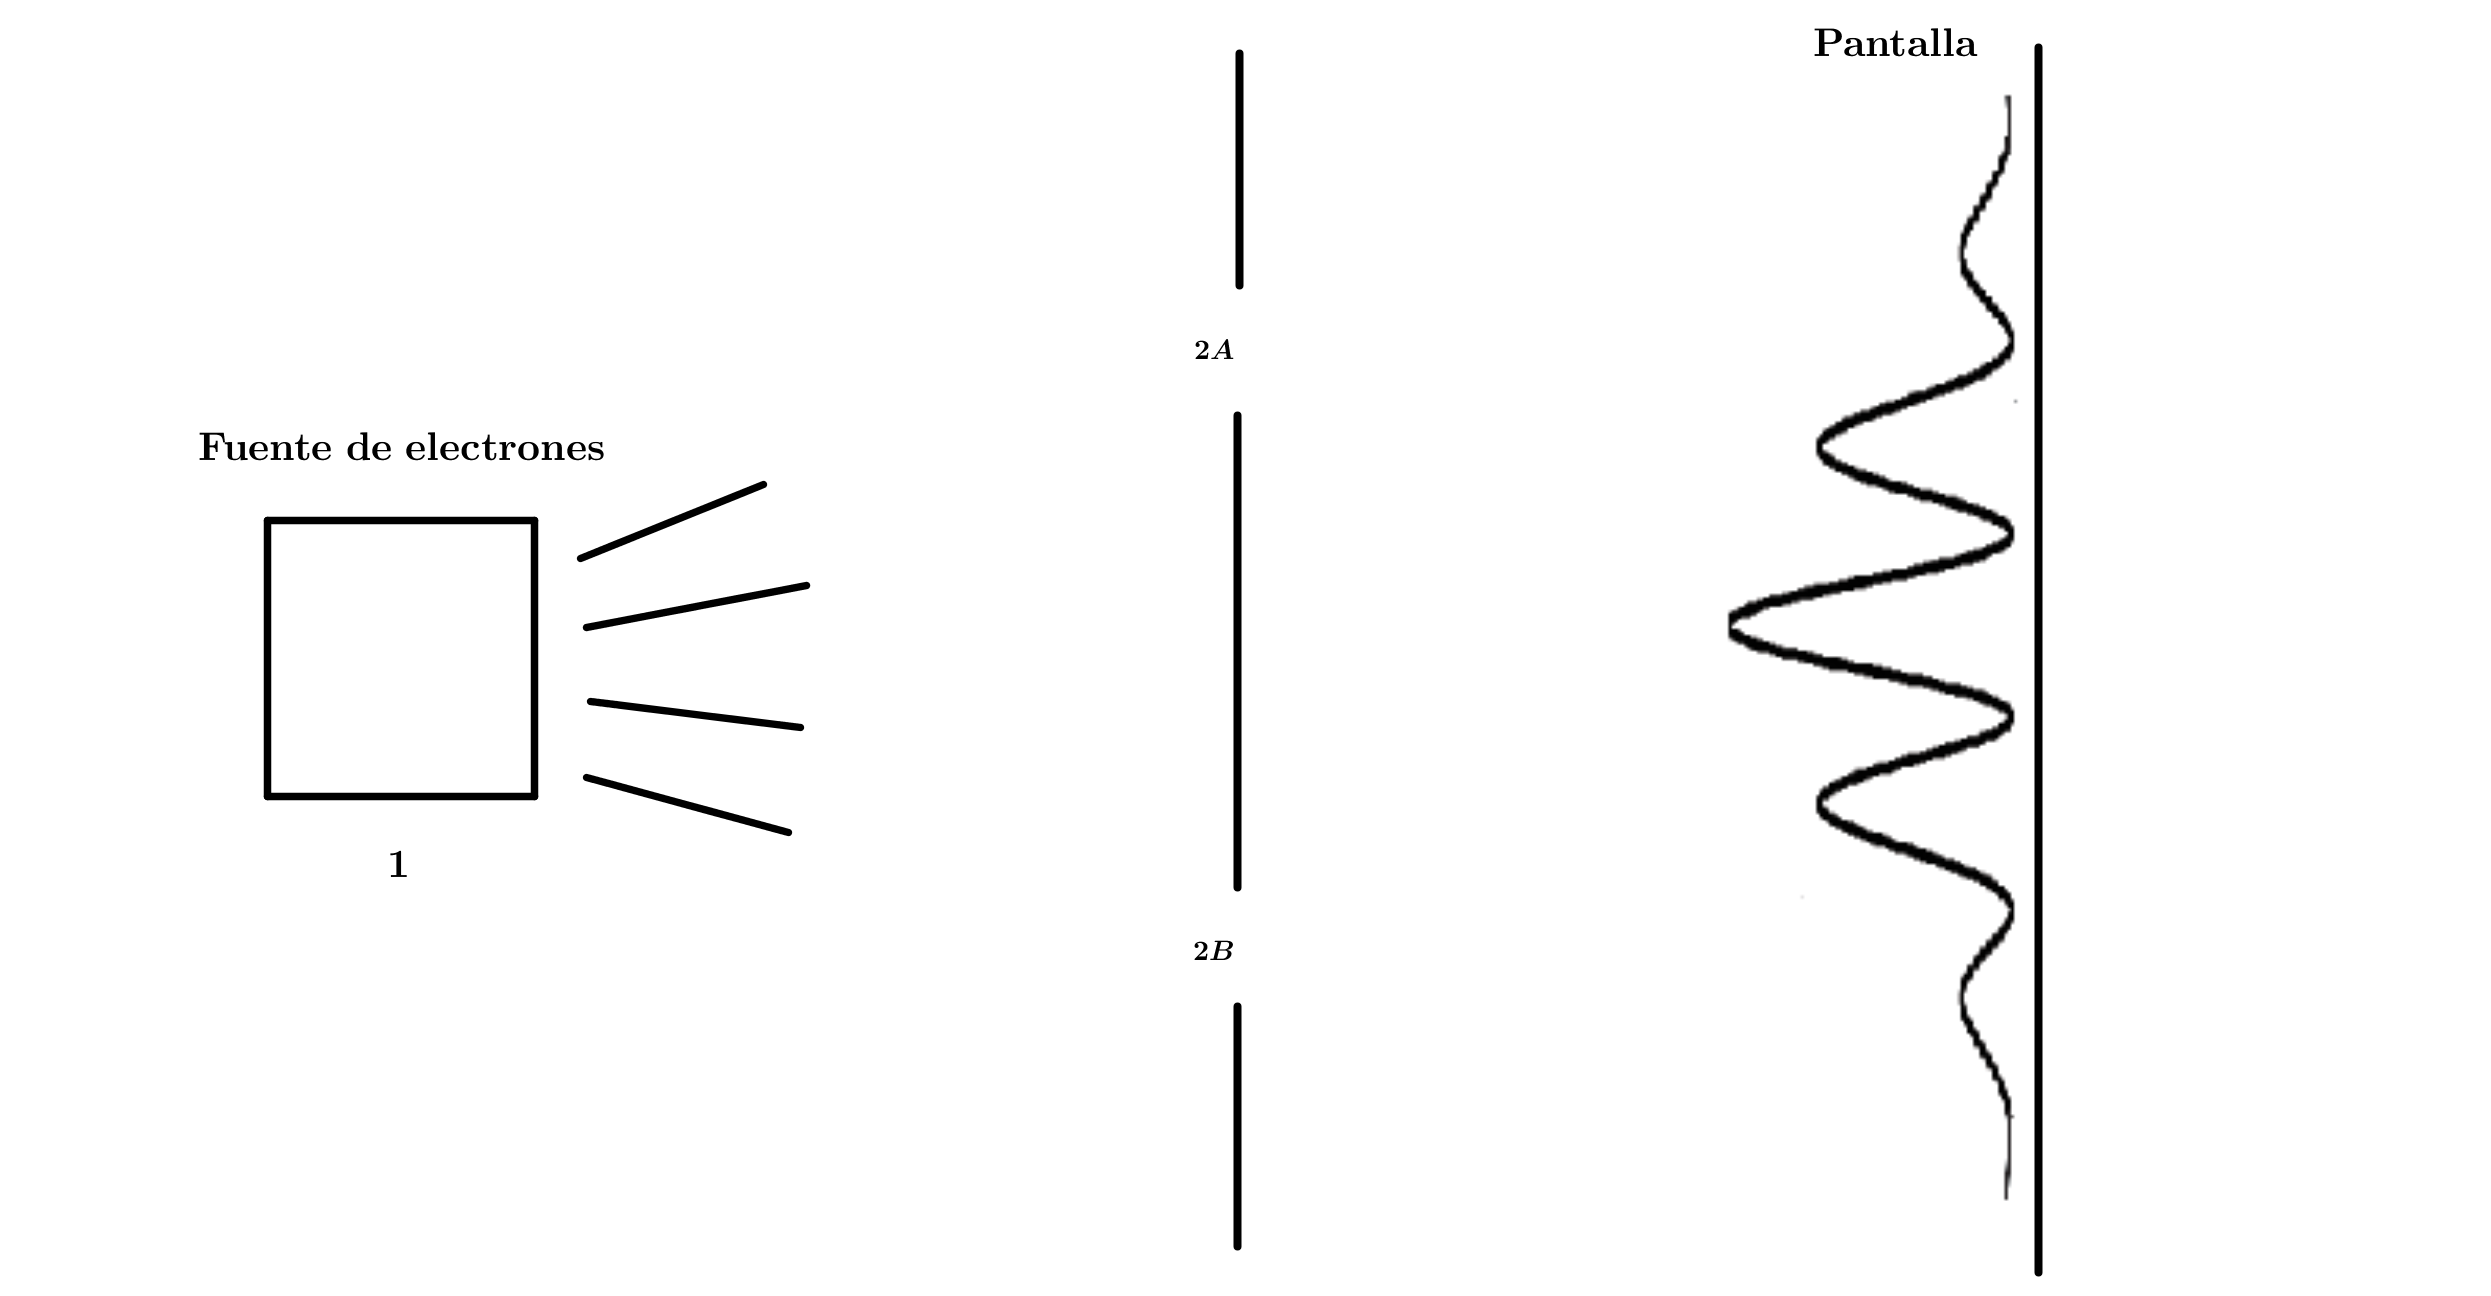
\includegraphics[width=9cm]{Imagenes/Fig1}
\caption[Esquema del experimento de la doble rendija]{Experimento de la doble rendija.}
\end{figure}
Si $K(2A,1)$ es la probabilidad de que un electrón pase por la rendija 2A, entonces podemos escribir:
\begin{equation}
K(3,1)=K(2A,1)K(3,2A)+K(2B,1)K(3,2B)
\end{equation}
Al tomar el módulo cuadrado de la expresión (2.5) se generarán los términos de interferencia necesarios para describir el patrón de difracción. No podemos decir que el electrón tomó un camino u el otro, de una manera más simple: este siguió todos los caminos posibles!

\section{La ecuacion de Schrodinger.}
En el cuadro de Schrodinger la evolución de un sistema cuántico afecta al ket que representa al estado del sistema, la ecuación que rige la dinámica del mismo es la \textbf{Ecuación de Schrödinger}
\begin{equation}
i\hbar\frac{\partial}{\partial t}|\psi\rangle_S=\hat{H}|\psi\rangle_S
\end{equation}
Sabemos que $\psi(q,t)=\langle q|\psi \rangle_S$ donde $|q\rangle$ son autoestados de la posición, la relacion entre el cuadro de Heisenberg y el de Schrödinger es $|\psi\rangle_H=e^{iHt/\hbar}|\psi\rangle_S$. Si definimos $|qt\rangle \equiv e^{iHt/\hbar}|q\rangle$, entonces $\psi (q,t)=\langle qt|\psi\rangle_H$.

Vamos a mostrar que $K(q_f,t_f;q_i,t_i)=\left\langle q_ft_f|q_it_i \right\rangle$, la relación de completez nos permite escribir:
\begin{eqnarray}
\nonumber \langle q_ft_f|\psi\rangle &=& \int\langle q_ft_f|q_it_i\rangle\langle q_it_i|\psi\rangle dq_i\\
&=& \int \langle q_ft_f|q_it_i\rangle \psi(q_i,t_i)dq_i
\end{eqnarray}
Y comparando (2.7) y (2.2), vemos que:
\begin{equation}
K(q_f,t_f;q_i,t_i)=\langle q_ft_f|q_it_i\rangle
\end{equation}
Así, el propagador es proporcional a la amplitud de probabilidad de transición entre el estado inicial $|q_it_i\rangle$ y final $|q_ft_f\rangle$. La idea ahora es expresar el propagador como una integral de trayectoria. Partamos el intervalo temporal $(t_i,t_f)$ en $n+1$ piezas de igual duración $\tau$, así:
\begin{equation}
\langle q_ft_f|q_it_i\rangle \int dq_1dq_2...dq_n\langle q_ft_f|q_nt_n\rangle \langle q_nt_n|q_{n-1}t_{n-1}\rangle...\langle q_1t_1|q_it_i\rangle
\end{equation}
Calculemos uno de estos elementos:
\begin{eqnarray}
\nonumber \langle q_{j+1}t_{j+1}|q_jt_j\rangle &=&\langle q_{j+1}|e^{-iHt_{j+1}/\hbar}e^{iHt_j/\hbar}|q_j=\langle q_{j+1}|e^{-i\tau H/\hbar}|q_j\rangle \hspace{0.4cm}\text{A primer orden,}\\
\nonumber &=&\langle q_{j+1}|1-i\tau H/\hbar|q_j\rangle=\delta(q_{j+1}-q_j)-i\tau\hbar\langle q_{j+1}|H|q_j\rangle\\
&=& \frac{1}{2\pi\hbar}\int dp\ \text{Exp}[\frac{ip}{\hbar}(q_{j+1}-q_j)]-\frac{i\tau}{\hbar}\langle q_{j+1}|H|q_j\rangle 
\end{eqnarray}	
Si asumimos que el Hamiltoniano es una función de $p$ y $q$de la forma: $H=\frac{p^2}{2m}+V(q)$, entonces:
\begin{eqnarray}
\nonumber \langle q_{j+1}|\frac{p^2}{2m}|q_j \rangle &=& \int dpdp\prime \langle q_{j+1}|p\prime\rangle\langle p\prime|\frac{p^2}{2m}|p\rangle \langle p|q_j \rangle\\
\nonumber &=&\int \frac{dpdp\prime}{2\pi\hbar}\ \text{Exp}[\frac{i}{\hbar}(p\prime q_{j+1}-pq_j)]\frac{p^2}{2m}\delta(p-p\prime)\\
&=& \int \frac{dp}{2\pi\hbar}\ \text{Exp}[\frac{i}{\hbar}p(q_{j+1}-q_j)]\frac{p^2}{2m}
\end{eqnarray}
De una manera similar:
\begin{eqnarray}
\nonumber \langle q_{j+1}|V(q)|q_j \rangle &=& V(\frac{q_{j+1}+q_j}{2})\langle q_{j+1}|q_j\rangle\\
\nonumber &=& V(\frac{q_{j+1}+q_j}{2})\delta(q_{j+1}-q_j)\\
\langle q_{j+1}|V(q)|q_j \rangle &=& V(\frac{q_{j+1}+q_j}{2})\int \frac{dp}{2\pi\hbar}\ \text{Exp}[\frac{i}{\hbar}p(q_{j+1}-q_j)]
\end{eqnarray}
Por tanto $\langle q_{j+1}|H|q_j\rangle=\int \frac{dp}{h}\ \text{Exp}[\frac{i}{h}p(q_{j+1}-q_j)]H(p,q)$ y:
\begin{equation}
\langle q_{j+1}t_{j+1}|q_jt_j\rangle=\frac{1}{h}\int dp_j\ \text{Exp}[\frac{i}{\hbar}[p_j(q_{j+1}-q_j)-\tau H(p_j,q_j)]]
\end{equation}
Finalmente:
\begin{equation}
\langle q_{f}t_{f}|q_it_i\rangle=\lim_{N \to \infty}\int\prod_{j=1}^{N}dq_j\prod_{j=0}^{N}\frac{dp_j}{h}\ \text{Exp}\left\{ \frac{i}{\hbar}\sum_{j=0}^{N}[p_{j}(q_{j+1}-q_{j})-\tau H(p_{j},q_{j})]\right\}
\end{equation}
En el continuo:
\begin{equation}
\langle q_{f}t_{f}|q_it_i\rangle=\int\frac{\mathcal{D}q\mathcal{D}p}{h}\text{Exp\ensuremath{\left\{ \frac{i}{\hbar}\int_{t_{i}}^{t_{f}}(p\dot{q}-H(p,q))dt\right\} }}
\end{equation}
En el continuo $q$ se vuelve una función de $t$ y la integral anterior, es una integral funcional. La expresión (2.15) es la integral de trayectoria para la amplitud de transición entre $(q_i,t_i)$ y $(q_f,t_f)$. Esta integral se hace sobre todas las posibles trayectorias en el espacio de fase y $q(t), p(t)$ son funciones y no operadores, sin embargo es natural preguntarse por la convergencia de (2.15), esto es algo no trivial, sin embargo, de ahora en adelante asumiremos que esta integral existe y converge. 	
\\
Si el Hamiltoniano es tal que $H=\frac{p^2}{2m}+V(q)$
\begin{equation}
\langle q_{f}t_{f}|q_it_i\rangle=\lim_{N \to \infty}\int\prod_{j=1}^{N}dq_j\prod_{j=0}^{N}\frac{dp_j}{h}\ \text{Exp}\left\{ \frac{i}{\hbar}\sum_{j=0}^{N}[p_{j}(q_{j+1}-q_{j})-\tau \frac{p_j^2}{2m}-V(q)\tau]\right\}
\end{equation}
Y sabiendo que: $\int_{-\infty}^{\infty}\text{Exp}[-ax^{2}+bx+c]dx=\text{Exp}[\frac{b^{2}}{4a}+c](\frac{\pi}{a})^{\frac{1}{2}}$, entonces:
\begin{equation}
\langle q_{f}t_{f}|q_it_i\rangle=\lim_{N\to\infty}[\frac{1}{h}(\frac{\text{\ensuremath{\pi\hbar}2m}}{\tau})^{\frac{1}{2}}]^{N}\int\prod_{1}^{N}dq_{j}\text{Exp}\left\{ \frac{i}{\hbar}\sum_{0}^{N}\left((\frac{q_{j+1}-q_{j}}{\tau})^{2}\frac{m}{2}-V\right)\tau\right\} 
\end{equation}
En el continuo:
\begin{equation}
\langle q_{f}t_{f}|q_it_i\rangle=\mathcal{N}\int\mathcal{D}q\text{Exp\ensuremath{\left\{ \frac{i}{\hbar}\int_{t_{i}}^{t_{f}}\mathcal{L}(q,\dot{q})dt\right\} }}
\end{equation}
Donde $\mathcal{L}(q,\dot{q})$ es el lagrangiano clásico, sin embargo esto solo pasa si asumimos una forma específica del Hamiltoniano, cuando esto no es asi se tiene una acción efectiva. En teorñia de campos por ejemplo esta descomposición solo se puede hacer en el caso de campos Abelianos.

 
\subsection{A Subsection}

Donec urna leo, vulputate vitae porta eu, vehicula blandit libero. Phasellus eget massa et leo condimentum mollis. Nullam molestie, justo at pellentesque vulputate, sapien velit ornare diam, nec gravida lacus augue non diam. Integer mattis lacus id libero ultrices sit amet mollis neque molestie. Integer ut leo eget mi volutpat congue. Vivamus sodales, turpis id venenatis placerat, tellus purus adipiscing magna, eu aliquam nibh dolor id nibh. Pellentesque habitant morbi tristique senectus et netus et malesuada fames ac turpis egestas. Sed cursus convallis quam nec vehicula. Sed vulputate neque eget odio fringilla ac sodales urna feugiat.

\section{El experimento de la doble rendija.}

\section{Campos escalares.}
\section{Campos fermiónicos.}
\section{Teorías Gauge y campos de Yang-Mills}
\section{La teoria de Yukawa}